
\section{Übersicht der Messung}

\begin{figure}[H]
\centering
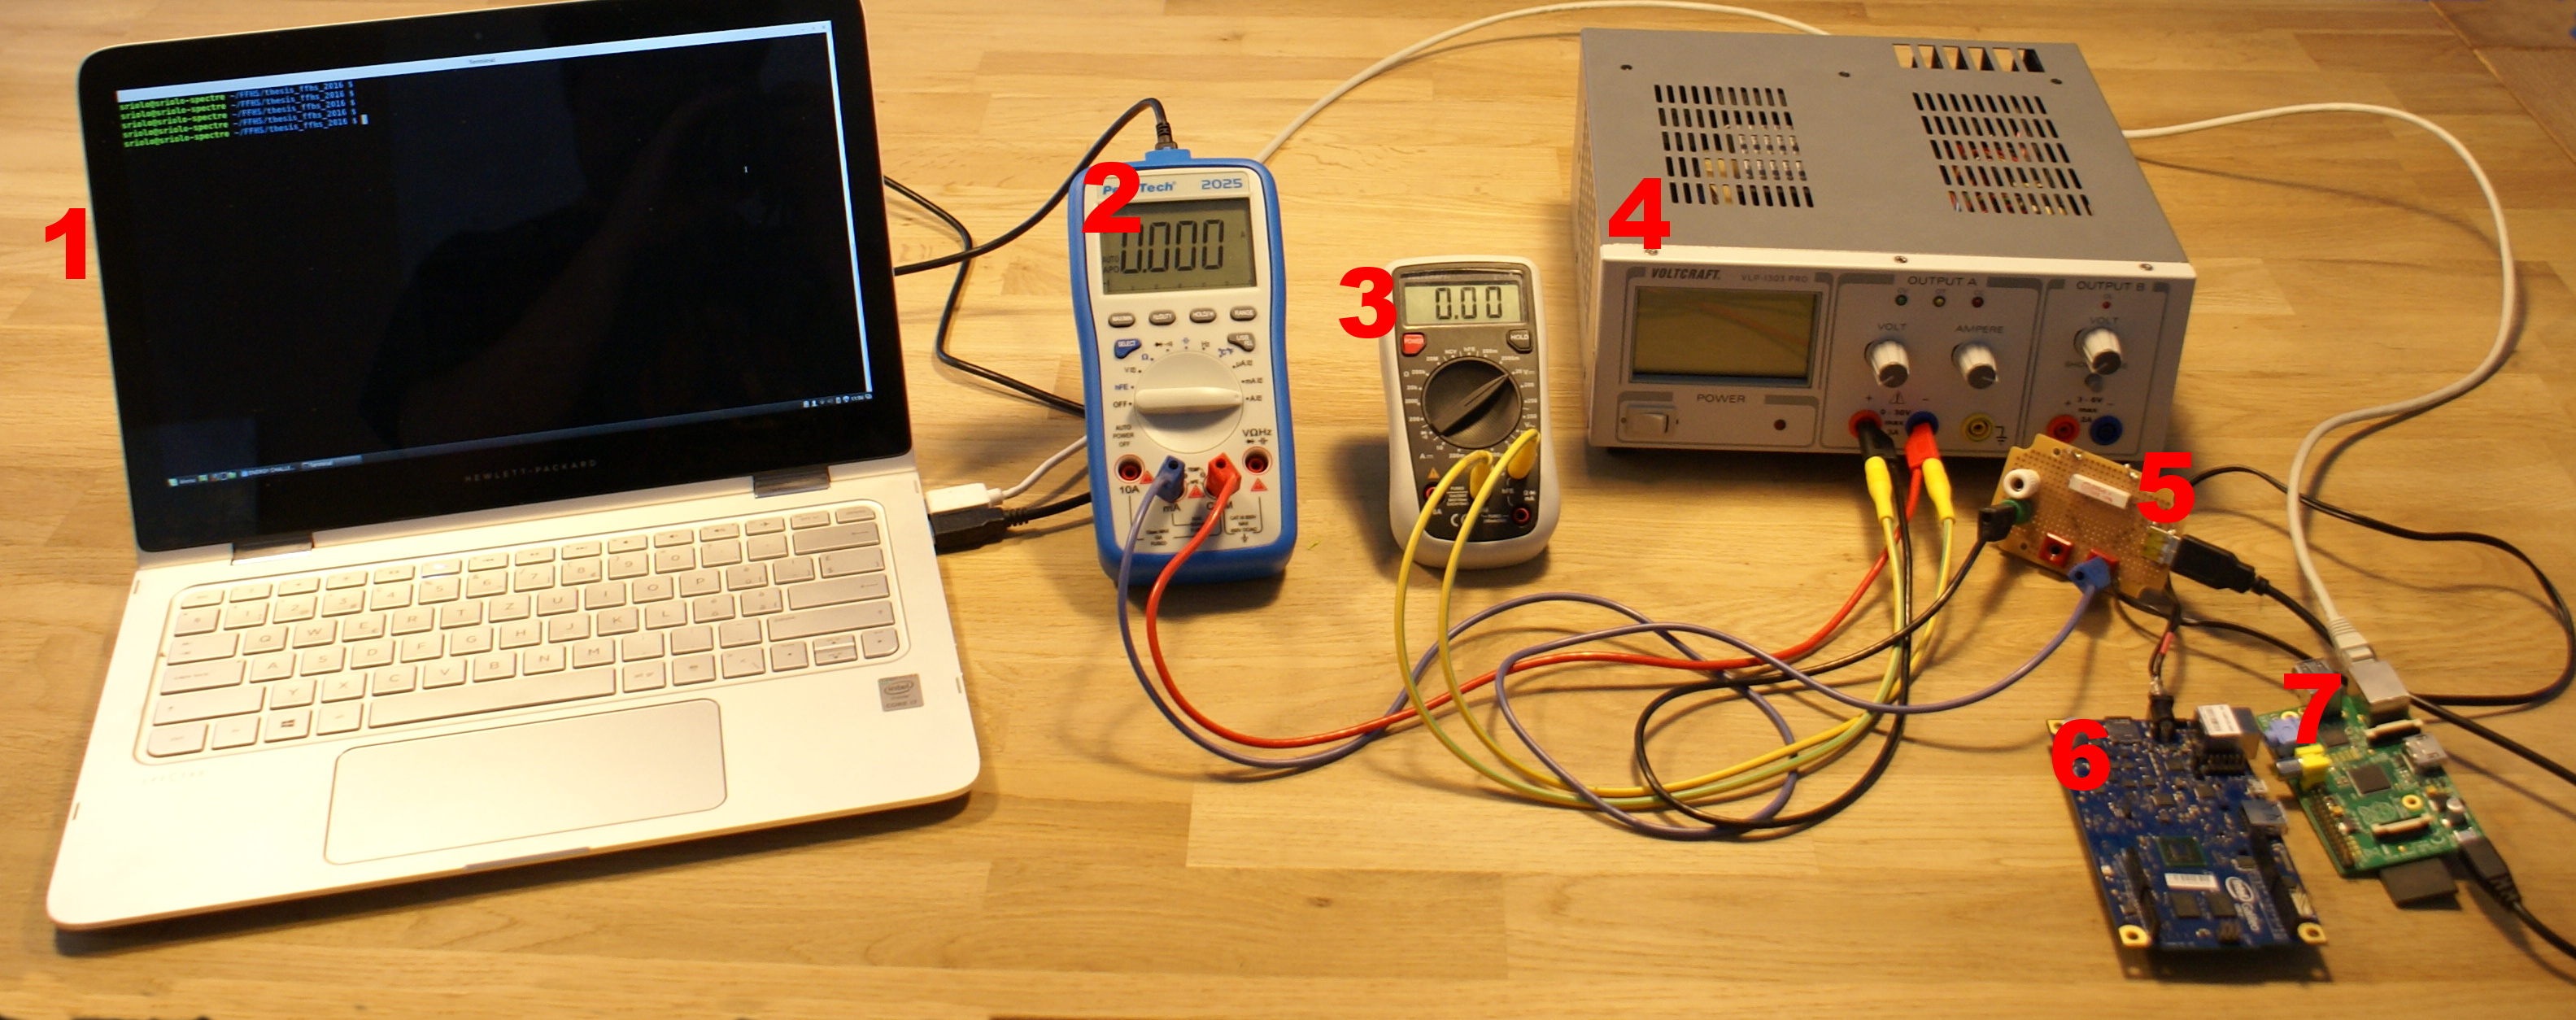
\includegraphics[width=1.0\textwidth]{images/setup.jpg}
\caption{Übersicht der Messung}
\label{fig:Setup}
\end{figure}

Für die Messung sind folgende Elemente notwendig die in der \autoref{fig:Setup} ersichtlich sind: 1.) Ein PC der die Benchmarks auf dem SoC ausführt und die gemessene Daten entgegennimmt. 2.) Messgerät der der Strom misst und die Daten über eine USB-Schnittstelle an den PC weiterleitetet. 3.) Optionales Messgerät, damit die Spannung des Spannungsreglers überprüft werden kann. 4.) Ein Spannungsregler der eine konstante Spannung sicherstellt. 5.) Ein Verteiler damit ein Galileo oder Raspberry Board angeschlossen werden kann. Ansonsten hat der Verteiler keine elektronische Eigenschaft. 6.) Das Galileo Board. 7.) Das Raspberry Board.

